\subsection{Framework}
Evan You ist der Gr\"under eines JavaScript Frameworks \textbf{Vue.js}\cite{Springer2017}. Vue.js ist ein clientseitiges Framework, mit dem Webanwendungen in JavaScript komponentenorientiert entwickelt werden k\"onnen. Dies bedeutet, dass die Anwendung in kleine Teile unterteilt wird, die miteinander kommunizieren und als eigenst\"andige Module laufen. Das Framework setzt die Implementierung einer Webanwendung mit dem Architekturmuster Model-View-ViewModel durch und bietet hierdurch eine schlanke, universelle, anpassungsf\"ahige und performante Implementierung\cite{Teufel2018}. Das Interesse an Vue.js ist in den letzten Jahren immer mehr gestiegen, was sich auch in den Google Trends zeigt\cite{GoogleTrends2018}.
\subsubsection*{Aufbau}
Der Aufbau gleicht dem von Angular.js oder React.js. Diese Frameworks werden in weiteren Abschnitten etwas genauer erl\"autert werden. Eine Anwendung besitzt mehrere Komponenten, die an sich einheitlich sind, aber von den anderen Komponenten zu trennen sind und \"uber eine bestimmte Schnittstelle kommunizieren. F\"ur die Benutzeroberfl\"ache wird \ac{HTML} benutzt, welche durch Attribute erweitert werden kann. Die Schnittstelle zur Kommunikation der Komponente wird an diese Attribute durch Datenbindung und Events realisiert. In diesem \ac{HTML} Dokument stellt Vue.js viele Hilfsmittel f\"ur Styling und Formulare bereit. Um weitere Funktionen hinzuzuf\"ugen, werden Plug-ins in die Anwendung eingebaut\cite{Springer2017}. Beispiele hierf\"ur sind vue-router oder vue-custom-element.
\begin{figure}[h] 
\centering
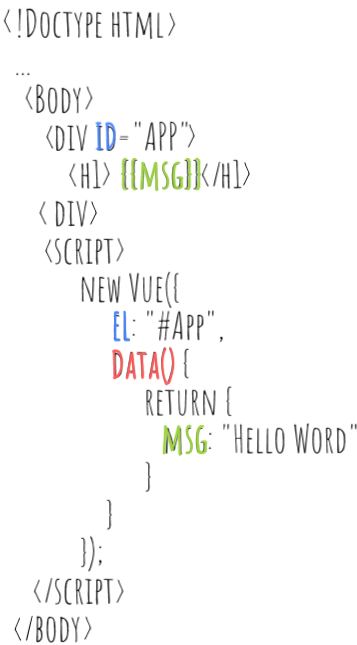
\includegraphics[scale=0.5]{fig/gettingStartedVue.PNG} 
\caption{Codebeispiel Initialisierung Vue}
\label{fig:CodeVueInit}
\end{figure} 
Zuerst muss ein Standard \ac{HTML} Dokument erstellt werden. Es enth\"alt ein \texttt{<head>} und ein \texttt{<body>} Tag. Innerhalb des \texttt{body} Tags wird ein \texttt{div} mit einer Identifikation erstellt, beispielsweise wie in Abbildung \ref{fig:CodeVueInit} mit \texttt{id=\grqq app\grqq{}}. Die Anwendung wird dort integriert. Um Daten wie einen String anzuzeigen, wird ein beliebiger Tag erstellt (zum Beispiel \texttt{h1}), der innerhalb einen Identifier besitzt, der in einer geschweiften Klammer (\texttt{<h1> \{\{msg\}\} </h1>}) steht. Um die \texttt{msg} mit einem String zu bef\"ullen, wird ebenfalls innerhalb des \texttt{body} Tags ein \texttt{<script>} Tag definiert. Hier wird eine Instanz der Vue erstellt. Die Instanz besitzt das Attribut \texttt{el}, das f\"ur die Identifikation zust\"andig ist, hei\ss{}t hier sollte \texttt{\#app} stehen. Des Weiteren hat die Vue Instanz eine \texttt{data()} Funktion, die Objekte, wie die \texttt{msg}, zur\"uck gibt.

\subsubsection*{Model-View-ViewModel}
Das Ausf\"uhren des Architekturmuster \ac{MVVM} in Vue.js hat eine deutliche und klare Abgrenzung der Komponenten und kann durch das einfache Beispiel in Abbildung \ref{fig:MVVMVue}  veranschaulicht werden.
\begin{figure}[h] 
\centering
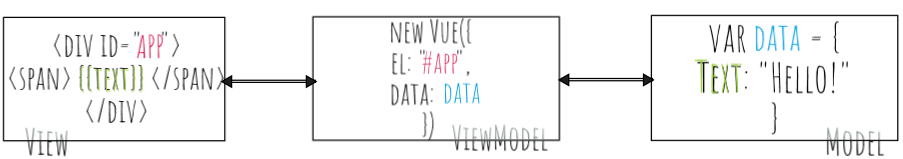
\includegraphics[scale=0.6]{fig/vueJSmvvm.PNG} 
\caption{MVVM in VueJS}
\label{fig:MVVMVue}
\end{figure} 
Die Benutzerschnittstelle, die dem Anwender dargestellt wird, wird in \ac{HTML} erfasst. In Vue.js wird dabei ein \textit{div} mit einer Identifikation, im Beispiel der Abbildung \ref{fig:MVVMVue} \texttt{app}, erstellt. In dem div soll ein Text stehen der durch das ViewModel \"ubergeben werden soll. Dieser ist, wie auch in Angular oder \"ahnlichen Templating Frameworks, mit zwei geschweiften Klammern geschrieben. 
Der Text, der an diese Stelle eingef\"ugt werden soll, wird im Model deklariert. Es wird ein Objekt erstellt, mit einem Attribut \texttt{Text}, in diesem Beispiel ein String. Das Attribut muss genauso bezeichnet werden wie das Wort innerhalb der geschweiften Klammer im \ac{HTML} Dokument.
Das Objekt wird an das ViewModel \"ubergeben und dort in die Vue Instanz \"ubertragen. In der Vue Instanz muss die Identifikation des \texttt{div} stehen und das Objekt, das an die Oberfl\"ache gegeben werden soll. Wenn das ViewModel die Instanz an das View \"ubergibt, erkennt die View die Identifikation und sucht im entsprechenden \ac{HTML} Dokument nach der passenden Identifikation. Ist das \texttt{div} gefunden, werden die Daten durchsucht und sobald dann das Attribut \texttt{Text} gefunden wurde, wird dies an der Stelle mit dem gleichen Attributsnamen eingesetzt.
